\documentclass[aspectratio=169,11pt]{beamer}
\usetheme{default}
\usecolortheme{seahorse}
\setbeamertemplate{navigation symbols}{}
\setbeamertemplate{footline}[frame number]
\setbeamerfont{frametitle}{series=\bfseries, size=\large}
\usepackage{booktabs}
\usepackage{graphicx}

\title{\textbf{Aims 1 and 2 update:}\\ measuring the language component in multilingual LLMs}
\author{Waiz Khan \\ \texttt{wkhan12@jh.edu}}
\date{July 2026 \\[2mm] \small 17 models $\cdot$ 122--128 languages $\cdot$
31 pre-registered predictions $\cdot$ 4/4 blind prospective test}

\begin{document}

\begin{frame}
\titlepage
\end{frame}

\begin{frame}{The question, in the proposal's own words}
\vspace{3mm}
\begin{quote}\large
``It is \textbf{not clear how strong the language component} in the
representation is, or should be\ldots'' \hfill (\S3.1.1)
\end{quote}
\vspace{4mm}
\begin{quote}\large
``At this point, \textbf{we have not singled out a specific metric}.''
\hfill (\S3.1.4)
\end{quote}
\vspace{6mm}
\centering This talk: that metric, built, validated, stress-tested.
\end{frame}

\begin{frame}{The answer: the Language-Factor Share (LFS)}
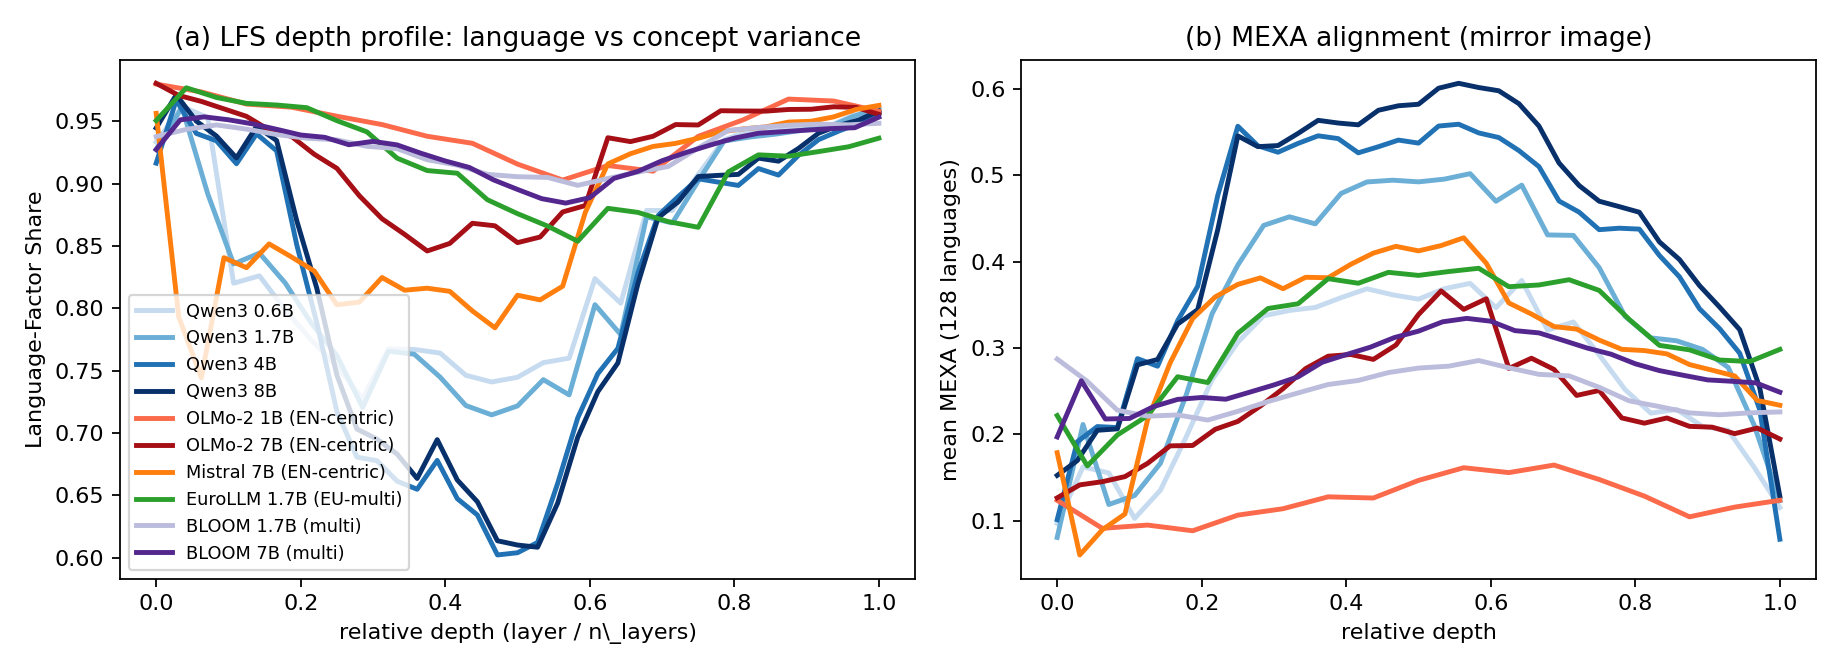
\includegraphics[width=\textwidth]{figs/fig1_lfs_depth_profile.png}
\vspace{1mm}
\small Per-layer variance share attributable to \emph{language identity} vs
\emph{meaning}. Every model funnels; the depth varies $0.04$--$0.34$: \textbf{a measurable, model-dependent quantity}. Family moves it more than scale (this grid).
\end{frame}

\begin{frame}{Your three-stage sketch has finer structure: two events}
\centering
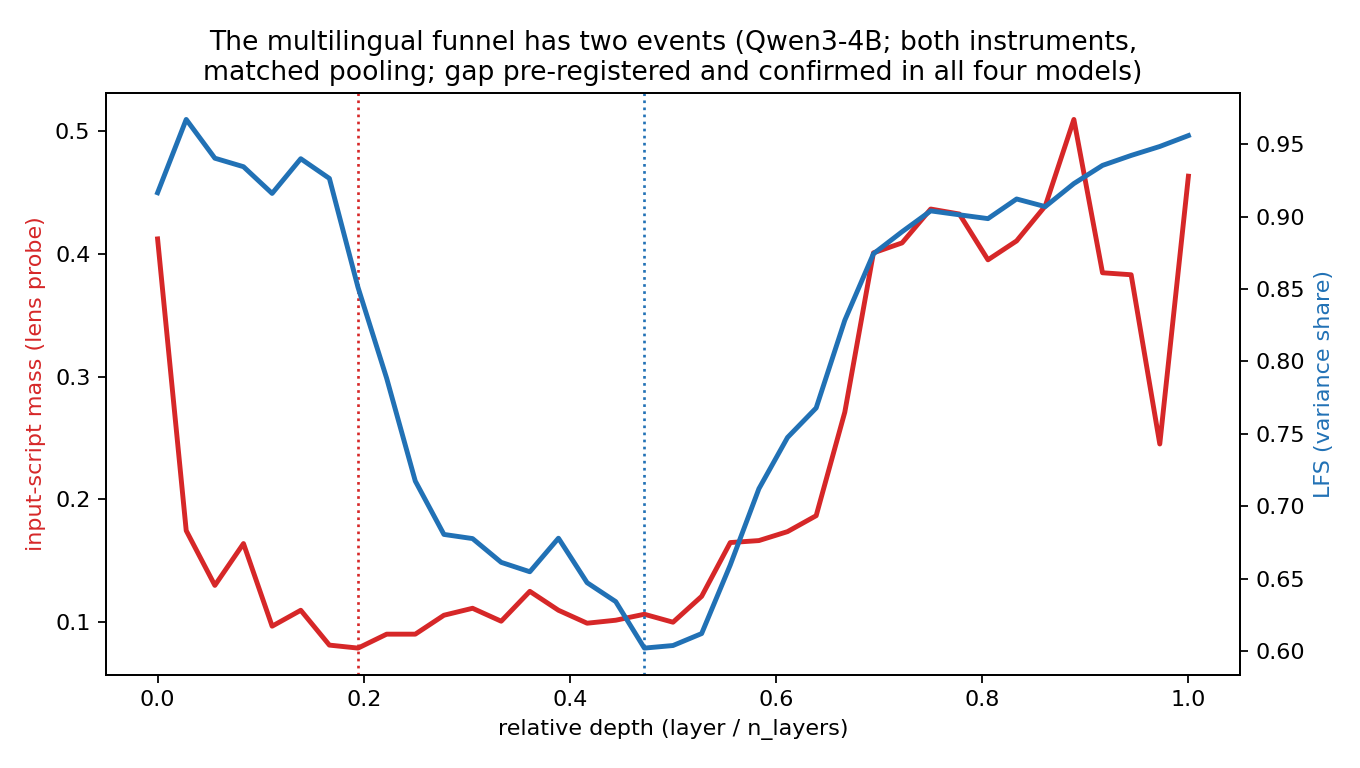
\includegraphics[width=0.72\textwidth]{figs/fig12_twoevents.png}
\vspace{1mm}

\small Script is abandoned \emph{early}; concepts converge \emph{mid}.
Pre-registered, confirmed twice, under matched pooling.
\end{frame}

\begin{frame}{Before the findings: how we checked our own results}
\begin{itemize}\itemsep=2mm
  \item My first hub estimate: latent-over-English $+1.04$. \textbf{I found
  the confound myself}; the corrected number is $+0.08$; still 113 to 124 of 127 languages by model.
  \item \textbf{31 pre-registered predictions, 21 passed; every failure
  documented} next to every success (several failures became new findings).
  \item \textbf{7 self-caught errors} with mechanisms in the report's ledger:
  a collapsed estimator withdrawn, a silently-unfair eval protocol caught,
  precision corruption, a gamed loss detected by the suite itself.
\end{itemize}
\vspace{2mm}
\centering\small The claims that follow survived all of this.
\end{frame}

\begin{frame}{On our grid, the standard validation number is roughly half confound}
\centering
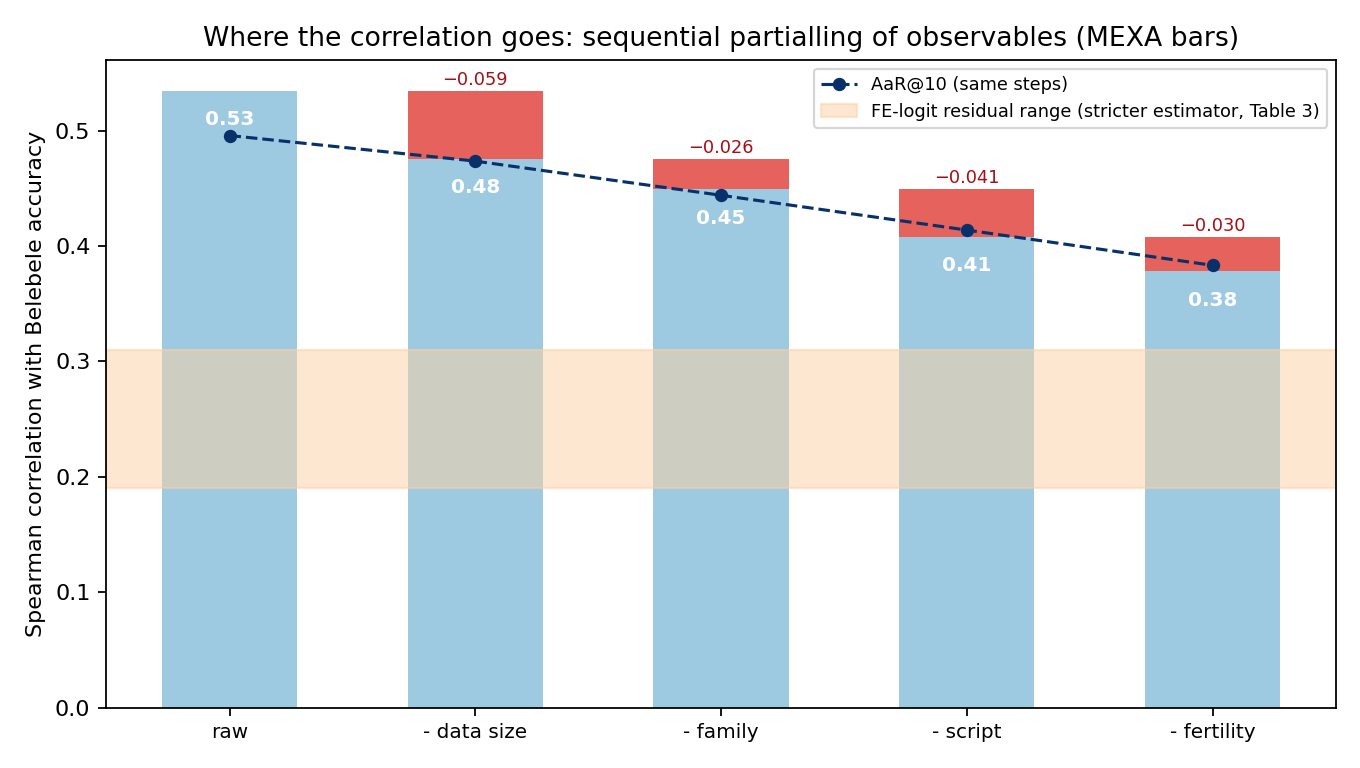
\includegraphics[width=0.66\textwidth]{figs/fig11_waterfall.png}
\vspace{1mm}

\small Data-rich languages score high on \emph{both} alignment and tasks.
\textbf{Confounder-adjusted validity}: partial out tokens, family, script, tokenizer; what survives is the metric's real signal.
\end{frame}

\begin{frame}{Confounder-adjusted results}
\centering
\begin{tabular}{lcc}
\toprule
 & vs.\ raw accuracy & vs.\ transfer residual \\
\midrule
AaR@10 (tail measure) & 0.50 & 0.23--0.31 \\
MEXA (reference) & 0.53 & 0.19--0.27 \\
\bottomrule
\end{tabular}
\vspace{4mm}

\small Estimator range $\rho \approx 0.19$--$0.31$; the July figure of about 0.59 on a benchmark-capable subset is withdrawn (not reproducible from any stored artifact).
\textbf{The measures are not ranked against each other; AaR's job is the failing tails that means hide.} MEXA is shown for reference. Preregistered prediction P4 passed on one held-out model and is not used as a ranking.
\end{frame}

\begin{frame}{Shared-space alignment predicts behavior, beyond observables}
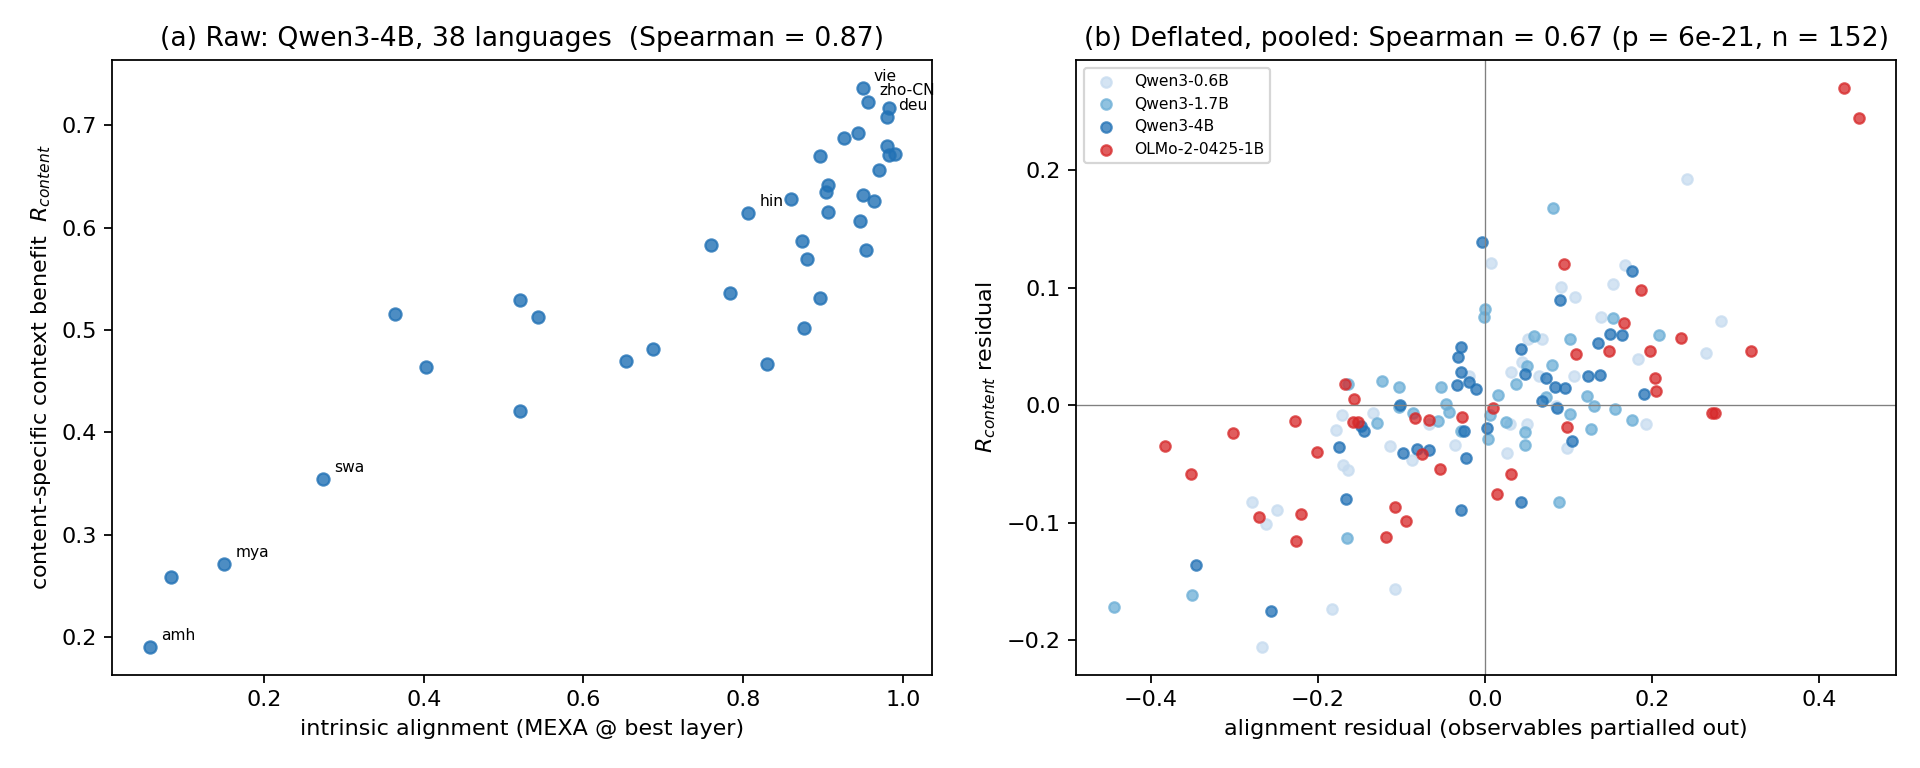
\includegraphics[width=\textwidth]{figs/fig10_b2scatter.png}
\vspace{1mm}
\small Alignment at the LFS-identified layer predicts how much the model \emph{uses} a foreign-language
context in generation: confounder-adjusted $\rho = 0.67$ (clustered CI $[0.55, 0.77]$;
wrong-document control rules out entity leakage).
\textbf{Observational.} Tested under intervention (Aim 2), the association
does not transfer.
\end{frame}

\begin{frame}{Why tails: the mean misleads}
\centering
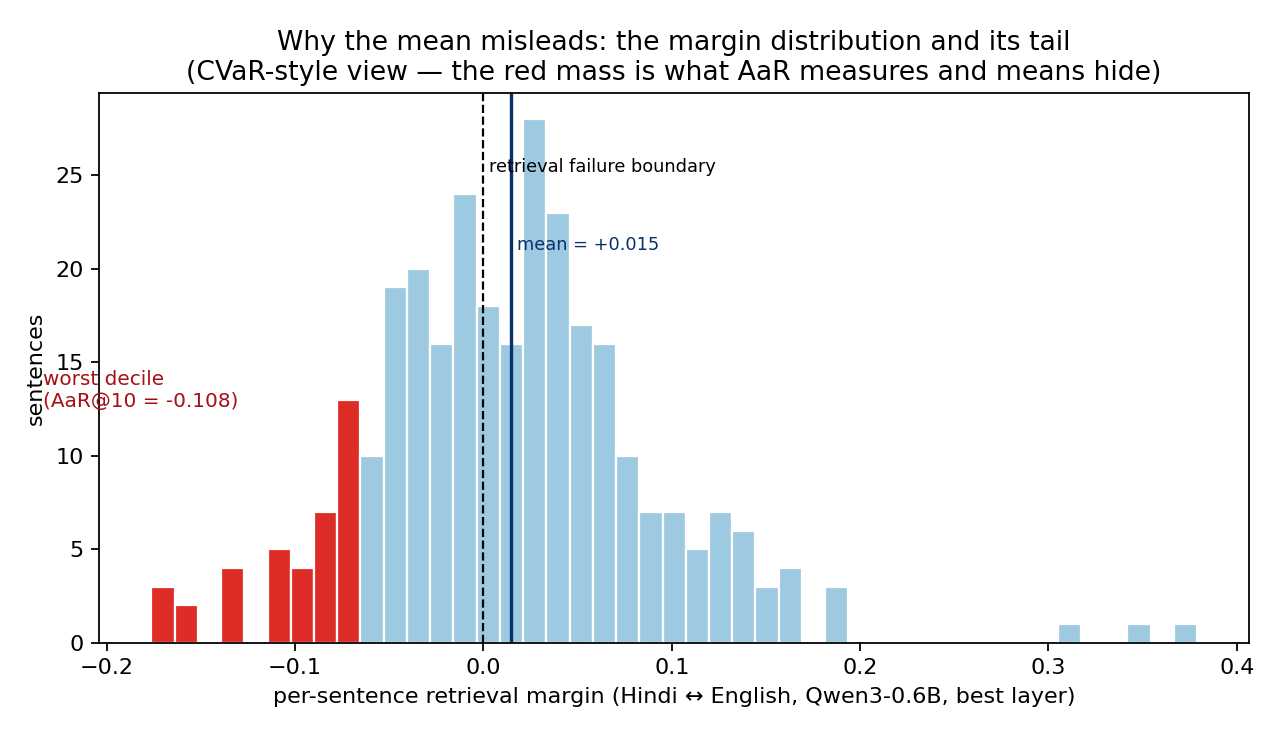
\includegraphics[width=0.68\textwidth]{figs/fig14_cvar.png}
\vspace{1mm}

\small Hindi: mean margin $+0.015$ (looks fine); worst decile $-0.108$
(failing). At $n{=}1500$: \textbf{40--50\% of languages in the best models
are mean-positive, tail-negative} (Qwen3-8B: Turkish $+0.13$ / $-0.26$).
The tail is \emph{semantic} (anaphora and culture-bound vocabulary), not entity noise. We read it.
\end{frame}

\begin{frame}{Generalization: pre-registered prospective test, 4/4 blind}
\small
\begin{tabular}{p{7.2cm}l}
\toprule
Prediction (frozen before running) & Result \\
\midrule
Unseen families match their recipe class (SmolLM2 shallow, Falcon3
intermediate) & PASS \\
Attribution criterion holds at 12 models & PASS \\
No validity collapse on unseen families (held-out \emph{exceeded} dev CI) &
PASS \\
Benchmark-capable $\Delta$ reproduces (retraction pre-committed) & PASS \\
\bottomrule
\end{tabular}
\vspace{3mm}

The design-circularity objection is substantially narrowed: the suite
classified two unseen families \textbf{under blind scoring} (one
benchmark-capable).
\end{frame}

\begin{frame}{We attacked the metric with calibrated faults, then measured its blind spots}
\centering

\includegraphics[width=0.78\textwidth]{figs/fig15_budget_composition.png}
\vspace{1mm}

\small Real cross-language misalignment is offset $+$ scale;
\textbf{rotation is at most 0.7\%} (14 models, $n{=}1500$; injected
rotations recovered exactly, so this is measured absence). The one attack
that is missed by every alignment metric tested (uniform collapse) is caught only
by our variance-preservation check.
\end{frame}

\begin{frame}{Aim 2: 28 conditions, and a defect in our own summary}
\begin{itemize}\itemsep=1.2mm
  \item \textbf{The objective \S3.2.2 specifies degenerates by 89\%.} A
  squared difference between matched word representations is minimized at
  $h=0$. Pre-registered, and it happened at all three seeds.
  \item \textbf{Neither LFS nor MEXA detects it.} Both are scale-invariant.
  The scale-collapsed condition posts the \emph{best} retrieval and \emph{best} tail
  alignment in the study; the sound condition gains nothing.
  \item \textbf{The components separate them by $20\times$.} The ratio
  $V_{\text{lang}}/(V_{\text{lang}}{+}V_{\text{concept}})$ divides out exactly
  the quantity that failed.
  \item \textbf{A collapse guard is necessary and not sufficient}: bounded
  hinge (0.81) against an unbounded objective (600). A $1000\times$ weight
  sweep saturates.
\end{itemize}
\vspace{1mm}
\small \textbf{Report the profile
$(V_{\text{lang}}, V_{\text{concept}}, \text{resid}, \lVert h\rVert)$, not the
share.} It catches every failure in this study; the share catches none.
\end{frame}

\begin{frame}{Asks, and what remains}
\textbf{Three things I'd value your input on:}
\begin{enumerate}\itemsep=1.5mm
  \item Where to go after the Aim-2 study: five objectives failed, and the
  collapse guard was necessary but not sufficient. Design the next one together?
  \item Venue, and ordering of pre-submission items (native-source
  replication, exact-count subset, FLORES).
  \item Coordination with adjacent work in the group.
\end{enumerate}
\vspace{3mm}
\small Boundaries, named: sentence-level, translated-news domain, one full
scaling family, proxy token counts, additive-share construct, and
observational validity that does not transfer under intervention. The last is now \emph{measured}: rotation is 0.06--0.2\% of real misalignment, and the
collapse attack that is missed by every alignment metric is caught by our
variance-preservation check. The point
of this work is not to hide uncertainty; it is to measure inside it.
\vspace{2mm}

\centering \footnotesize Full technical report (methods, statistics, and error ledger) and release-ready code available.
\end{frame}

\end{document}
